\documentclass{article} % For LaTeX2e
\usepackage{nips15submit_e,times}
\usepackage{hyperref}
\usepackage{url}
\usepackage{natbib}
%\documentstyle[nips14submit_09,times,art10]{article} % For LaTeX 2.09
\usepackage{amsthm}
\usepackage{amsmath}
\usepackage{amssymb}
\usepackage{graphicx}
\usepackage{epstopdf}
\usepackage{array}
\usepackage{xspace}
\usepackage{enumerate}


% For algorithms
\usepackage{algorithm}
\usepackage{algorithmic}

\title{Deterministic Independent Component Analysis}


\author{
Ruitong Huang \\
Department of Computing Science\\
University of Alberta \\
Edmonton, AB T6G2E8 Canada\\
\texttt{ruitong@ualberta.ca} \\
\And
Andr\'as Gy\"orgy \\
Department of Electrical and Electronic Engineering\\ 
Imperial College London\\ 
South Kensington Campus, London SW7 2BT, UK \\
\texttt{a.gyorgy@imperial.ac.uk} \\
\And
Csaba Szepesv\'ari \\
Department of Computing Science\\
University of Alberta \\
Edmonton, AB T6G2E8 Canada\\
\texttt{szepesva@ualberta.ca}
}

% The \author macro works with any number of authors. There are two commands
% used to separate the names and addresses of multiple authors: \And and \AND.
%
% Using \And between authors leaves it to \LaTeX{} to determine where to break
% the lines. Using \AND forces a linebreak at that point. So, if \LaTeX{}
% puts 3 of 4 authors names on the first line, and the last on the second
% line, try using \AND instead of \And before the third author name.

\newcommand{\fix}{\marginpar{FIX}}
\newcommand{\new}{\marginpar{NEW}}
\newcommand{\iid}{i.i.d.\xspace}
\newcommand{\ra}{\rightarrow}
\newcommand{\real}{\mathbb{R}}
\renewcommand{\natural}{\mathbb{N}}
\DeclareMathOperator{\pol}{Poly}
\newcommand{\poly}[1]{\pol\left(#1\right)}
\newcommand{\E}{\mathbb{E}}

\newtheorem{lemma}{Lemma}[section]
\newtheorem{thm}[lemma]{Theorem}
\newtheorem{claim}[lemma]{Claim}
\newtheorem{cor}[lemma]{Corollary}
\newtheorem{example}[lemma]{Example}
\newtheorem{prop}[lemma]{Proposition}
\theoremstyle{definition}
\newtheorem{definition}[lemma]{Definition}
\newtheorem{remark}[lemma]{Remark}
\newtheorem*{solution}{Solution}
\newtheorem{note}[lemma]{Note}
\newtheorem{problem}[lemma]{Problem}
\newtheorem{assumption}[lemma]{Assumption}
\nipsfinalcopy % Uncomment for camera-ready version

\begin{document}


\maketitle

\begin{abstract}
We study independent component analysis with noisy observations in a deterministic framework. We present a consistent, polynomial-time algorithm to reconstruct the mixing matrix with a data-dependent error bound. In contrast to earlier work, our results hold without any stochastic assumptions on the source signals and the observation noise. When applied
to the standard i.i.d.\ stochastic ICA model, 
our algorithm, for the first time in the literature, achieves a reconstruction error that vanishes at a $1/\sqrt{T}$ rate using $T$ observations and scales only polynomially with the natural parameters of the problem.  
\end{abstract}

\section{Introduction}
Independent Component Analysis (ICA)
%, as a main tool of blind source separation, 
has received much attention in the past decades. 
In the standard ICA model one can observe a $d$-dimensional vector $X$ that is a linear mixture of $d$ independent variables $(S_1,\ldots, S_d)$ with Gaussian noise:
\begin{equation}
\label{eq:stoch-ICA}
X = AS+\epsilon,
\end{equation}
where $\epsilon \sim \mathcal{N}(0,\Sigma)$ is a $d$-dimensional Gaussian noise with zero mean and covariance matrix $\Sigma$, and $A$ is a nonsingular $d \times d$ mixing matrix. 
The goal of the observer is to recover (separate) the source signals and the mixing matrix given several independent and identically distributed (\iid) observations from the above model based on the information on the independence only.
The ICA literature is vast in both practical algorithms and theoretical analyses; 
we refer to the book of \citet{comon2010handbook} for a comprehensive survey.
In practice, ICA is also known to work well for unmixing the mixture of various deterministic signals. 
One of the classical demonstrations of ICA is showing that two periodic signals can be well recovered from their mixtures \citep{HyvOja00}.
Such an example is shown in Figure~\ref{fig:demo}. 
\begin{figure}[h]
\label{fig:demo}
\centering
	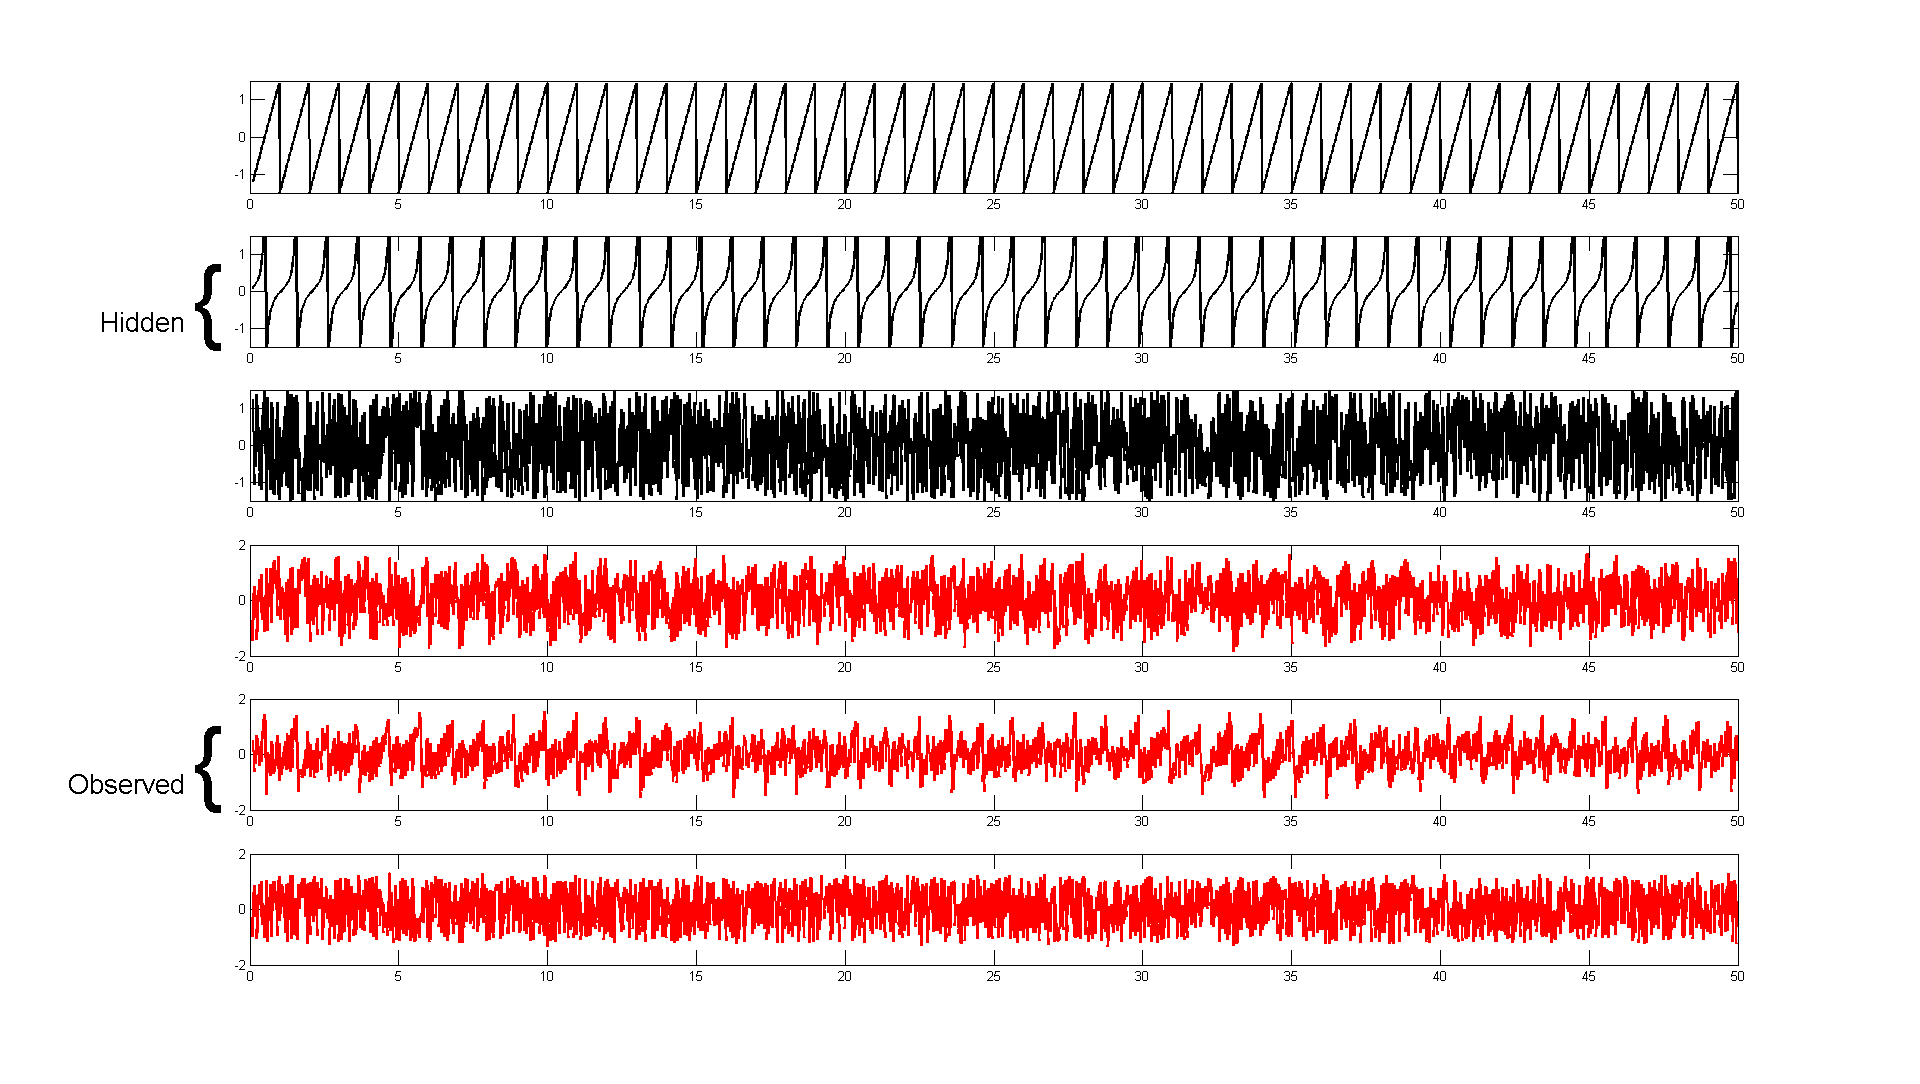
\includegraphics[width = 0.49\linewidth]{demo_source}
	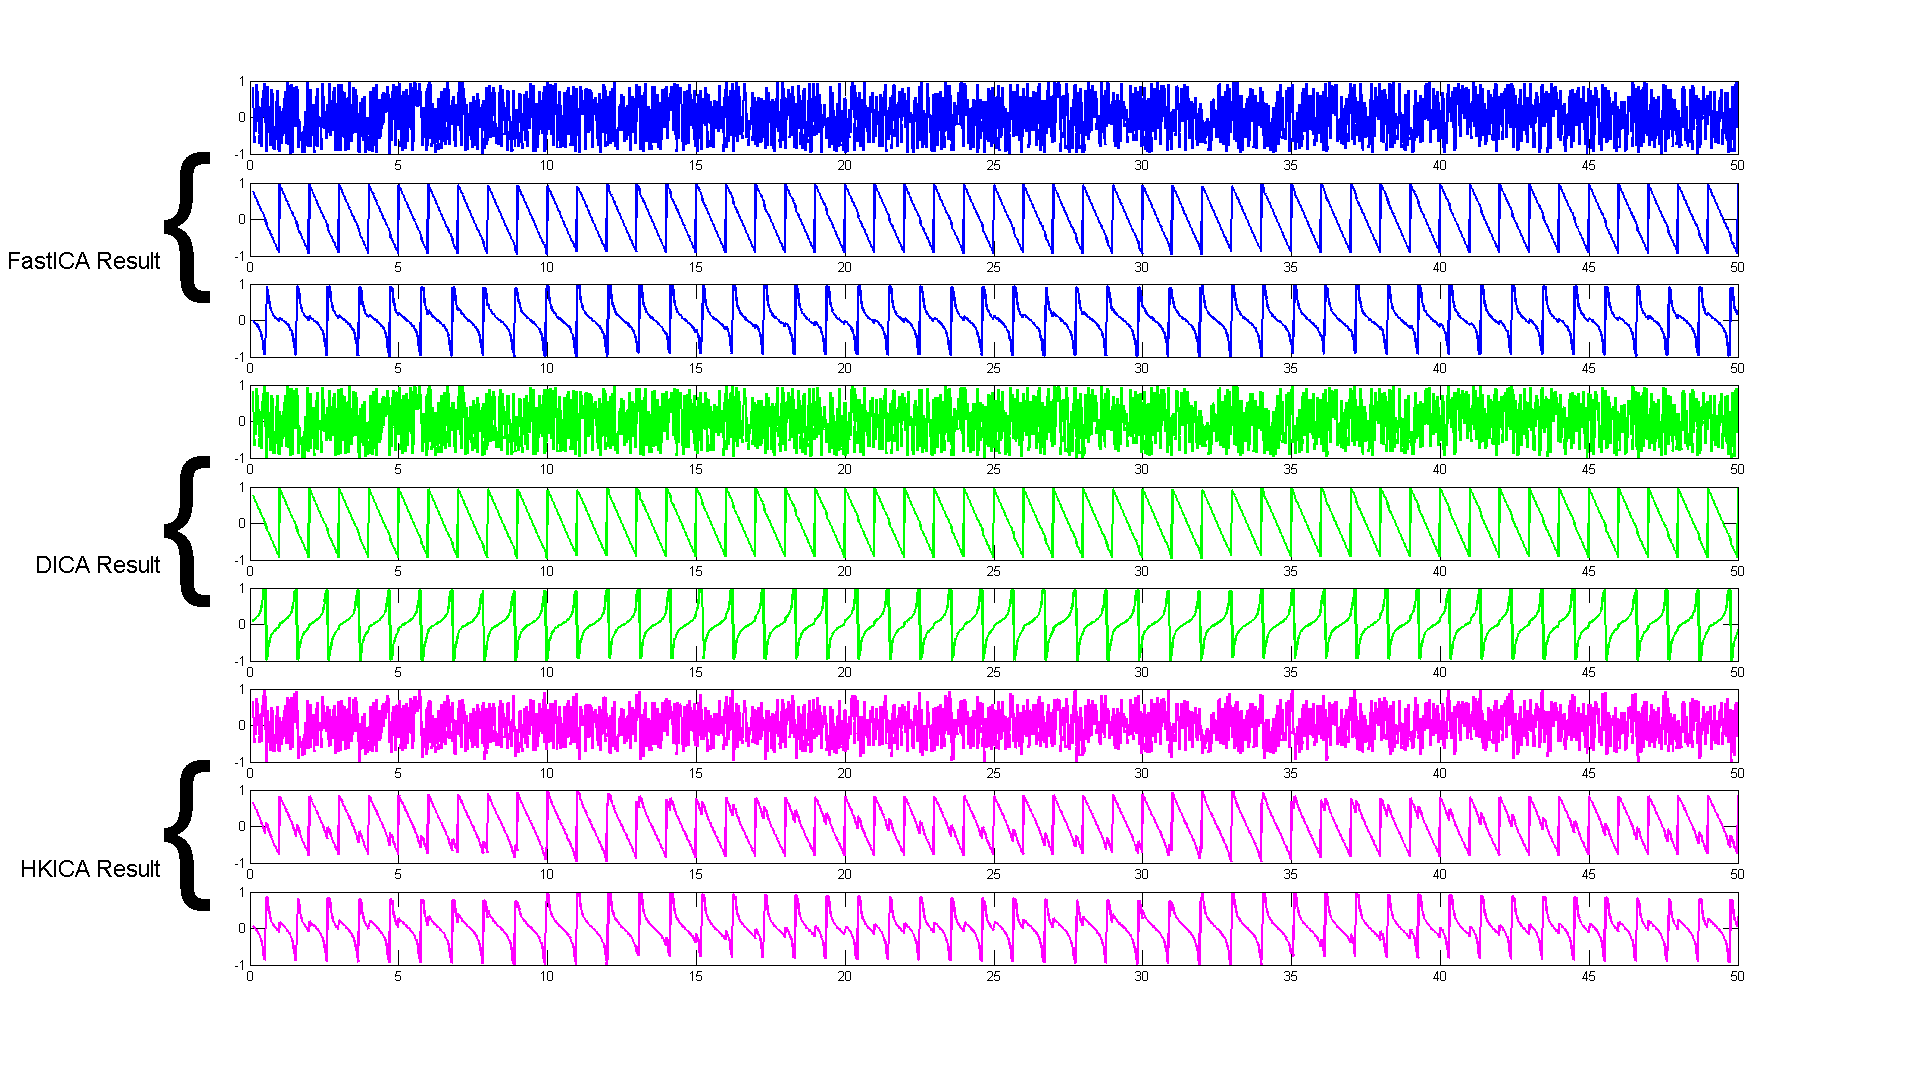
\includegraphics[width = 0.49\linewidth]{demo_res}
\caption{Example of ICA: The black signals are the source signals, red ones observed signals (left). The right figure shows the reconstructed (and rescaled) signals from FastICA, HKICA, and DICA (3 different ICA algorithms, see Section \ref{subsec:relatedWorks} and \ref{sec:DICA} for details ) after sampling $As(t)$ at 2500 uniformly spaced points in the interval $[0,50]$.}
\end{figure}
This phenomenon suggests that the usual probabilistic notion is unsatisfactory if one wishes to have a deeper understanding of ICA.  

The main contribution of our paper is to analyze ICA algorithms in a deterministic framework. 
Our deterministic analysis helps investigate this curious phenomenon. Our result can be applied to more general setting without losing any generality to the traditional stochastic setting. 
Formally, instead of observing $T$ \iid samples from \eqref{eq:stoch-ICA}, the observations and the source signals are defined by the functions  $x:\natural \ra \real^d$ and $s:\natural \ra \real^d$ as $d$-dimensional deterministic functions. 
We study the question that to what extent can the mixture of signals be separated. 
We proposed a \emph{provable polynomial-time} algorithm that has \emph{no free parameter} for the noisy ICA model.
The analysis of the algorithm's performance is reduced to perturbation analysis, which depends on how much the observation function is deviated from the stochastic model. 
We proposed a data-dependent measure for such deviation based on the empirical distribution of data.
It can be shown that this measure converges to 0 in a rate of $O(\sqrt{T})$ for $T$ \iid samples from  \eqref{eq:stoch-ICA}.
Therefore when applied to the stochastic model, our algorithm is guaranteed to correctly reconstruct the mixing matrix $A$.

The rest of this paper is organized as follows: 
Our main results are highlighted in Section~\ref{sec:main}.
The polynomial-time algorithms underlying these results are developed through Section~\ref{sec:DICA}.
Due to space limit, proofs and experimental results are presented in the full version of the paper \citep{HuGySz15}.

\subsection{Related Works}
\label{subsec:relatedWorks}
Perheps the most popular approach to the ICA problem is the FastICA algorithm \citep{hyvarinen1999fast}. 
Great progress has been made to analyze FastICA theoretically \citep{tichavsky2006performance,oja2006fastica,ollila2010deflation,dermoune2013fastica,wei2014convergence}.
In particular, recently \citet{miettinen2014fourth} showed that in the noise-free case (i.e., when $X = AS$), the error of FastICA (when using a particular forth-moments-based contrast function) vanishes at a rate of $1/\sqrt{T}$ where $T$ is the sample size.
In addition, several other methods have been shown to achieve similar error rates in the noise-free setting \citep[e.g.,][]{eriksson2003characteristic,samarov2004nonparametric,chen2005consistent,chen2006efficient}.
However, to our knowledge, no similar finite sample results are available in the noisy case.

On the other hand, promising algorithms based on moment methods are available in the noisy case that make significant advances towards provably efficient and effective ICA algorithms, albeit fall short of either providing a complete solution or providing rigorous proofs. \citep{anandkumar2012tensordecomposition,anandkumar2012method, arora2012provable, hsu2013learning, goyal2014fourier}
In particular, the results of \citep{arora2012provable} and \cite{goyal2014fourier} depend on some  unspecified parameters ($\beta$ in the paper of \citep{arora2012provable} and $\sigma$ in the paper of \citep{goyal2014fourier}) that are belong some specific range, making their algorithms impossible to tune.
A common problem faced by the other methods (\citep{anandkumar2012tensordecomposition,anandkumar2012method,hsu2013learning}) is a minimal gap of the eigenvalues, which may result in an exponential dependence on the number of source signals $d$. 
Recently, \citet{vempala2014max} proposed an ICA algorithm based on an elegant, recursive version of the method of \citet{goyal2014fourier} that avoids dealing with the aforementioned minimal gap; however, they still need an oracle to set the unspecified parameter of \citet{goyal2014fourier}.

The problem of separating mixture of deterministic signals are also consider in \citep{kirimoto2011separation} and \citep{forootan2013separation}. But the analysis is restricted to particular signals, while our result is applicable to general ones. 
\subsection{Notation}
We denote the set of real and natural numbers by $\real$ and $\natural$, respectively.
A vector $v \in K^d$ for a field $K$ is assumed to be a column vector.
Let $\|v\|_2$ denote its $L_2$-norm, and for any matrix $Z$ let $\|Z\|_2=\max_{v:\|v\|_2=1}{\|Z v\|_2}$ denote the corresponding induced norm. Denote the maximal and minimal singular value of $Z$ by $\sigma_{\max}(Z)$ and  $\sigma_{\min}(Z)$, respectively. Also, let $Z_i$ and $Z_{i:}$ denote the $i$th column and, resp., row of $Z$.
For a tensor (including vectors and matrices) $T$, its Frobenious norm (or $L_2$ norm) $\|T\|_F$  is defined as the square root of the sum of the square of all the entries.  
For a vector $v=(v_1,\ldots,v_d) \in K^d$, $\vert v \vert$ is defined coordinatewise, that is $\vert v \vert=(\vert v_1 \vert,\ldots,\vert v_d\vert)$. 
The transpose of a vector/matrix $Z$ is denoted by $Z^\top$, while the inverse of the transpose is denoted by $Z^{-\top}$.  
The outer product of two vectors $v, u \in K^d$ is denoted by $u\otimes v=u v^\top$. 
$v^{\otimes k}$ denotes the $k$-fold outer product of $v$ with itself, that is, $v\otimes v\otimes v \ldots \otimes v$, which is a k-dimensional tensor.
Given a $4$-dimensional tensor $T$, we denote the matrix $Z$ by $T(\eta,\eta,\cdot , \cdot)$ that is generated by marginalizing the first two coordinates of $T$ on the direction $\eta$, that is,
$Z_{i,j} = \sum_{k_1,k_2 = 1}^{d} \eta_{k_1} \eta_{k_2} T_{k_1,k_2,i,j}$. (Similar definitions for marginalizing different coordinates of the tensor.)
For a real vector $v$ and some real number $C$, $v \le C$ means that all the entries of $v$ are at most $C$. 
The bold symbol $\boldsymbol{1}$ denotes a vector with all entries being $1$ (the dimension of this vector will always be clear from the context).
Finally, $\poly{\cdot,\cdots,\cdot}$ denotes a polynomial function of its argument.

\section{Main Results}
\label{sec:main}
In this paper, we consider the problem that given $x(t), t\in [T]$, to what extent we can reconstruct the true mixing matrix $A$, as shown in Theorem \ref{thm:finalRes}.
Assume that we can observe the $d$ dimensional mixed signal $x(t) \in \real^d, t \in [T]:=\{1,2,\ldots,T\}$ generated by  
\begin{equation}
\label{eq:ICA}
x(t) = As(t)+\epsilon(t),
\end{equation}
where $A$ is a $d\times d$ nonsingular mixing matrix,  $s:[T] \to [-C,C]^d$ is a bounded, $d$-dimensional source function for some constant $C \ge 1$. , and $\epsilon:[T] \to \real^d$ is the noise function. 
We measure the performance of the algorithm by the reconstruction error of the mixing matrix $A$, as follows.
\[
d(\hat{A}, A) = \inf_{
		\substack{\pi \in \mathrm{Perm}([d]) \\ c\in \real^d}} 
		\max_{k} || c_k A_{:\pi(k)} - A_{:k} ||_2\,,
\]
where $\hat{A}$ is the reconstructed mixing matrix and $\mathrm{Perm}([d])$ is the set of all the permutations. 

We will denote the $i$th component of $s$ by $s_i$. 
Furthermore, we will use the notation $\sigma_{\min}=\sigma_{\min}(A)$ and
$\sigma_{\max}=\sigma_{\max}(A)$.
For any $t,k \ge 1$ and a function $u:[t] \to \real^k$, we introduce the empirical distribution $\nu_t^{(u)}$ defined by
$\nu_t^{(u)}(B)=\tfrac{1}{t}|\{\tau \in [t]: u(\tau) \in B\}|$ for all Borel sets $B \subset \real^k$.
Fix some product distribution $\mu= \mu_1\otimes \ldots \otimes \mu_d$ over $\real^d$ 
such that $\E_{S_i\sim\mu_i}[S_i]=0$ and $\kappa_i := \vert \E_{S_i\sim \mu_i}[S_i^4] - 3\left(\E_{S_i\sim \mu_i}[S_i^2]\right)^2 \vert \neq 0$. Let
$K$ denote the diagonal matrix $\text{diag}(\kappa_1,\cdots,\kappa_d)$, and define $\kappa_{\min}=\min_{i} \kappa_i$.

To measure the distance of $\nu_T^{(s)}$ from $\mu$, define the following family of ``distances'' to measure the closeness of two distributions: Given two distributions $\nu_1$ and $\nu_2$ over $\real^d$, let $D_k(\nu_1,\nu_2) = \sup_{f\in\mathcal{F}} |\int f(s)d\nu_1(s) - \int f(s)d\nu_2(s)|$, where $\mathcal{F}=\{f:\real^d \to \real : f(s)=\prod_{j=1}^k s_{i_j}, 1 \le i_1,\ldots,i_k \le d\}$ is the set of all monomials up to degree $k$.
Also let $D_k(\nu)  = \min_{\mu} D_k(\mu, \nu)$ where the minimization of $\mu$ is taken over the set of all the product measures. 

We also need to measure how approximately $s$ and $\epsilon$ are 0 mean, how Gaussian the noise function $\epsilon$ is, and lastly how independent $s$ and $\epsilon$ are. Let 
\begin{align*}
G = &  \max_{1\le t\le T}  \Huge{\{} \, \| \E_{S_i\sim \nu_t^{(s_i)}} [S_i] \|_F,\quad \| \E_{Y \sim \nu_t^{(\epsilon)}} [Y] \|_F, \\
& \quad  \max_{\|\eta\| \le 1} \Bigl\| \left(\E_{Y\sim \nu_t^{(\epsilon)}} [Y^{\otimes4}] - (\E_{Y\sim \nu_t^{(\epsilon)}} [Y^{\otimes2}])^{\otimes 2}\right)(\eta,\eta,\cdot,\cdot)  - 2 (\E_{Y\sim \nu_t^{(\epsilon)}} [Y^{\otimes2}])^{\otimes 2}(\eta,\cdot,\eta,\cdot)\Bigr\|_F, \\
& \quad \max_{
	\substack{i_1,i_2,j_1,j_2 \ge 0 \\ i_1+i_2+j_1+j_2 \le 4}}
 \| \E_{S\sim \nu_t^{(s)}} [(AS)^{\otimes i_1}\!\otimes \E_{Y\sim \nu_t^{(\epsilon)}} [Y^{\otimes j_1}] \!\otimes (AS)^{\otimes i_2}] \\
& \quad \quad \quad \quad - \E_{(S, Y)\sim \nu_t^{(s, \epsilon)}} [(AS)^{\otimes i_1}\!\otimes Y^{\otimes j_1}\!\otimes (AS)^{\otimes i_2}]  \|_F, \\
& \quad \max_{
	\substack{i_1,i_2,j_1,j_2 \ge 0 \\ i_1+i_2+j_1+j_2 \le 4}}
\| \E_{Y\sim \nu_t^{(\epsilon)}} [Y^{\otimes j_1} \otimes \E_{S\sim \nu_t^{(s)}} [(AS)^{\otimes i_1}] \otimes Y^{\otimes j_2}] \\
& \quad \quad \quad \quad - \E_{(S, Y)\sim \nu_t^{(s, \epsilon)}} [ Y^{\otimes j_1}\otimes (AS)^{\otimes i_1}\otimes Y^{\otimes j_2}] \|_F \, \Huge{\}}.
\end{align*}
Also, let 
\[
L = \max_{1\le t\le T} \left( \| \E_{Y\sim \nu_t^{(\epsilon)}} [Y^{\otimes 2}] \|_F,\, \| \E_{Y\sim \nu_t^{(\epsilon)}} [Y^{\otimes 3}] \|_F \right).
\]

Now we are ready to state our main result. 
\begin{thm}
\label{thm:finalRes} Consider the ICA problem \eqref{eq:ICA}. There exists an algorithm that estimates the mixing matrix $A$ from $T$ samples of $x$ such that (i) the computational complexity of the algorithm is $O(d^3 T)$; and (ii) with probability at least $1-\delta$, there exists a permutation $\pi$ and constants $\{c_1,\ldots,c_d\}$, such that for all $1\le k\le d$,
\[
\| c_k\hat{A}_{\pi(k)} - A_k\|_2 \le \mathcal{C} \min\left(D_4(\nu_T)+ G^2 +G, \Theta \right),
\]
where $\mathcal{C}$ and $\Theta$ are problem depedent constant, polynomial in $(\sigma_{\max}, 1/\sigma_{\min}, 1/\kappa_{\min},1/\delta, d, C, L)$ and $\hat{A}$ is the output of the algorithm.

In particular, in the traditional stochastic setting, if $S$ has distribution $\mu$ and
\[
T \ge \poly{d, \frac{1}{\kappa_{\min}}, \frac{1}{\delta}, C, \sigma_{\max}, \frac{1}{\sigma_{\min}}, \|\Sigma\|_2},
\]
then, with probability at least $1-\delta$, there exists a permutation $\pi$ and constants $\{c_1,\ldots,c_d\}$, such that for all $1\le k\le d$,
\begin{align*}
 \| c_k\hat{A}_{\pi(k)} - A_k\|_2 \le 
& \frac{\poly{C, \sigma_{\max}, \frac{1}{\sigma_{\min}}, \frac{1}{\kappa_{\min}},\frac{1}{\delta}, d}}{\sqrt{2T}}.
\end{align*}
\end{thm}

\if0
\subsection{Assumptions about the data}
\label{subsec:assumptions}
\begin{assumption}
\label{ass:gauss}
Assume there exists a constant $L$ and a function $g:\natural\rightarrow \real$ such that $g(t) \to 0$ as $t \to \infty$ and
\begin{enumerate}[(i)]
\item $\| \E_{S_i\sim \nu_t^{(s_i)}} [S_i] \|_F,\, \| \E_{Y \sim \nu_t^{(\epsilon)}} [Y] \|_F \le g(t)$; $\| \E_{Y\sim \nu_t^{(\epsilon)}} [Y^{\otimes 2}] \|_F,\, \| \E_{Y\sim \nu_t^{(\epsilon)}} [Y^{\otimes 3}] \|_F \le L$;
\item $\Bigl\| \left(\E_{Y\sim \nu_t^{(\epsilon)}} [Y^{\otimes4}] - (\E_{Y\sim \nu_t^{(\epsilon)}} [Y^{\otimes2}])^{\otimes 2}\right)(\eta,\eta,\cdot,\cdot)  - 2 (\E_{Y\sim \nu_t^{(\epsilon)}} [Y^{\otimes2}])^{\otimes 2}(\eta,\cdot,\eta,\cdot)\Bigr\|_F\le g(t)\|\eta\|_2^2$.
\end{enumerate}
Here $L$ and the function $g$ may depend on $\{A,\Sigma,C,d\}$.
\end{assumption}
\begin{assumption}
\label{ass:independence}
Assume the source signal function and the noise function are `independent' up to the 4th moment in the sense that for any $i_1,i_2,j_1,j_2 \ge 0$ such that $i_1+i_2+j_1+j_2 \le 4$,  
\[
 \| \E_{S\sim \nu_t^{(s)}} [(AS)^{\otimes i_1}\!\otimes \E_{Y\sim \nu_t^{(\epsilon)}} [Y^{\otimes j_1}] \!\otimes (AS)^{\otimes i_2}]
- \E_{(S, Y)\sim \nu_t^{(s, \epsilon)}} [(AS)^{\otimes i_1}\!\otimes Y^{\otimes j_1}\!\otimes (AS)^{\otimes i_2}]  \|_F 
 \le g(t),
\]
\[
\| \E_{Y\sim \nu_t^{(\epsilon)}} [Y^{\otimes j_1} \otimes \E_{S\sim \nu_t^{(s)}} [(AS)^{\otimes i_1}] \otimes Y^{\otimes j_2}]- \E_{(S, Y)\sim \nu_t^{(s, \epsilon)}} [ Y^{\otimes j_1}\otimes (AS)^{\otimes i_1}\otimes Y^{\otimes j_2}] \|_F 
\le g(t), % \le L/\sqrt{t},
\]
for the same function $g$ in Assumption \ref{ass:gauss}, where $(s,\epsilon)$ is the function obtained by concatenating $s$ and $\epsilon$ together.  
\end{assumption}
\begin{remark}
Assumption \ref{ass:gauss} (i) forces that the average of $s$ and $\epsilon$ decay to 0 at a rate of $g(t)$,
and that both the second and third moments of the noise be bounded.
Assumption \ref{ass:gauss} (ii) basically says that the induced measure of the noise function $\epsilon$ has 0 kurtosis in the limit.
Assumption \ref{ass:independence} is to guarantee that the source signals and the noise be approximately independent.
\end{remark}
\fi
\section{A deterministic ICA Algorithm}
\label{sec:DICA}
The algorithm is inspired by \citet{hsu2013learning}, \citet{arora2012provable}, and \citet{frieze1996learning} using a quasi-whitening procedure:
For any $p\ge 1$, $\eta\in \real^d$, and distribution $\nu$ over $\real^d$,
let 
$m_p^{(\nu)}(\eta) = \E_{X\sim \nu}[ (\eta^\top X)^p ],\, f_{\nu}(\eta) = \tfrac1{12} \left( m_4^{(\nu)}(\eta) - 3 m_2^{(\nu)}(\eta)^2 \right)$.
One can show that $\nabla^2 f_\mu(\psi)=A K D_{\psi} A^\top$ where $D_{\psi} =\text{diag}\left((\psi^{\top}A_1)^2,\cdots, (\psi^{\top}A_d)^2\right)$,
and so $B= AK^{1/2}D_{\psi}^{1/2}R^{\top}$ for some orthonormal matrix $R$. Defining $T_i=\nabla^2 f_\mu(B^{-\top} \phi_i)$, one can calculate that
$T_i=A K^{1/2} D_\psi^{-1/2} \Lambda_i A^\top$ where $\Lambda_i =\text{diag}\left( (\phi_i^\top R_1)^2,\ldots,(\phi_i^\top R_d)^2 \right)$ and $R_i$ denote the $i$th column of $R$.
Then $M=T_1 T_2^{-1} = A\Lambda A^{-1}$ with $\Lambda=\Lambda_1 \Lambda_2^{-1}=\text{diag}\left( \left(\frac{\phi_1^\top R_1}{\phi_2^\top R_1}\right)^2,\ldots,\left(\frac{\phi_1^\top R_d}{\phi_2^\top R_d}\right)^2 \right)$. Thus, $A_i$ are again the eigenvectors of $M$.
Note that the eigenvalues of $M$ are defined in terms of the orthogonal matrix $R$,
and so it is easy to handle the resulting minimum spacing
\begin{equation}
\label{def:gammaR}
\gamma_R =  \min_{i,j: i\neq j} \left\vert \left(\frac{\phi_1^{\top}R_i}{\phi_2^{\top}R_i}\right)^2 - \left(\frac{\phi_1^{\top}R_j}{\phi_2^{\top}R_j}\right)^2 \right\vert.
\end{equation}
We show in the full version \citep{HuGySz15} %Lemma~\ref{lem:ConstantProb} in the appendix 
that, among others,  $\gamma_R \ge\frac{\delta}{2d^2}$ with probability at least $1-\delta$.
The resulting algorithm, called Deterministic ICA (DICA), is shown in Algorithm \ref{alg:DICA}. 
\begin{algorithm}
\caption{Deterministic ICA (DICA)}
\label{alg:DICA}
\begin{algorithmic}[1]
\INPUT $x(t)$ for $1\le t \le T$. 
\OUTPUT An estimation of the mixing matrix $A$. 
\STATE Sample $\psi$ from a $d$-dimensional standard Gaussian distribution;
\STATE Evaluate $\nabla^2\hat{f}(\psi)$, \\
%\quad where $\hat{m_p}(\eta) = \frac{1}{T}\sum_{k=1}^{T} (\eta^{\top}g(k))^p$, and $\hat{f}(\eta) = \frac{1}{12}\big(\hat{m_4}(\eta) - 3\hat{m_2}(\eta)^2 \big)$;
\STATE Compute $\hat{B}$ such that $\nabla^2\hat{f}(\psi) = \hat{B}\hat{B}^{\top}$;
\STATE Sample $\phi_1$ and $\phi_2$ independently from the standard Gaussian distribution;
\STATE Compute $\hat{T}_1 =\nabla^2\hat{f}(\hat{B}^{-\top}\phi_1)$ and  $\hat{T}_2 =\nabla^2\hat{f}(\hat{B}^{-\top}\phi_2)$;

\STATE Compute all the eigenvectors of $\hat{M} = \hat{T}_1\left(\hat{T}_2\right)^{-1}$, $\{\mu_1,\ldots,\mu_d\}$;
\STATE Return $\hat{A} = \{\mu_1,\ldots,\mu_d\}$.
\end{algorithmic}
\end{algorithm}

\subsubsection*{Acknowledgments}
This work was supported by the Alberta Innovates Technology Futures and NSERC.
\bibliographystyle{plainnat}
\bibliography{DICA}
\end{document}
